%----------------------------------------------------------------------------
\chapter{Szemmozgások}\label{sect:osztalyozas}
%----------------------------------------------------------------------------

\begin{verse}
\begin{flushright}
\emph{A szív érez, a szem kutat} \\
\dots
\end{flushright}
\end{verse}

A szemmozgások többsége -- így a későbbi vizsgálatok szempontjából fontosak is -- a retinán elhelyezkedő sárgafolt (\emph{fovea centralis}, lásd \figref{eyediag} ábra) helyzetének megváltoztatására szolgál. A látóideg kivezetése mellett elhelyezkedő sárgafolton csak tömötten egymás mellé rendeződött csapok találhatók. A csapok jó fényviszonyok mellett nagyon magas felbontásban képesek színek gazdag skáláját feldolgozni, ezért a legélesebb látás a sárgafoltra vetített kép esetén lehetséges. Érthető tehát, hogy a sárgafoltot olyan pozícióba célszerű mozgatni, hogy a figyelem tárgyának képe ide vetüljön. Az ehhez szükséges pozicionáló típusú szemmozgások közé tartoznak a \emph{szakkádok}, a \emph{lassú követések}, és -- bár meglepőnek tűnik -- a \emph{fixációk} is, ezekkel a fejezet további szakaszaiban részletesebben foglalkozok.

\begin{figure}[!ht]
\centering
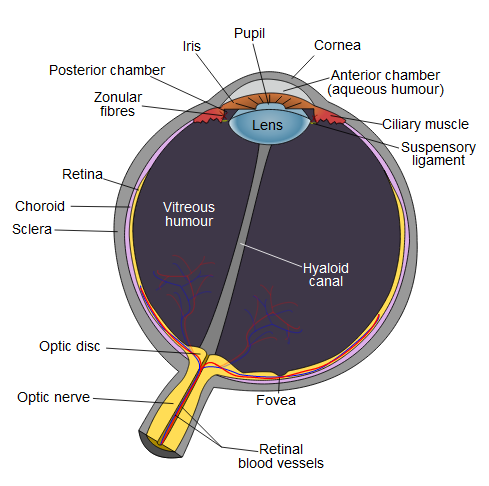
\includegraphics[width=100mm, keepaspectratio]{figures/eye_diagram.png}
\caption{Az emberi szem felépítése. Forrás: \url{http://en.wikipedia.org/wiki/Eye}}
\label{fig:eyediag}
\end{figure}

A \emph{fovea} pozicionálását elősegítő mozgások mellett természetesen más is szerepet kap a kívánt kép előállításában. A teljesség igénye nélkül, ilyenek például a szem divergenciáját illetve konvergenciáját beállító mozgások (mélységérzékelés), valamint azok a reflexszerű mozgások, amelyek az egyensúlyszervvel összhangban beállítják a szemeket a fej térbeli orientációjának megfelelően.

\bigskip

A fejezet \sectref{osztalyok} szakaszában sorra veszem, és bemutatom a pozicionáló típusú szemmozgások alapjait, a mérnöki megközelítésből jelentéktelen részleteket mellőzve. Végül a \sectref{mozg_osszegzes} szakaszban összefoglalom a megszerzett ismereteket, valamint hogy a megismert mozgások milyen követelményeket, illetve korlátozásokat támasztanak a realizálandó rendszer tervezése során.

%,,,,,,,,,,,,,,,,,,,,,,,,,,,,,,,,,,,,,,,,,,,,,,,,,,,,,,,,,,,,,,,,,,,,,,,,,,,,
\section{Osztályozás}\label{sect:osztalyok}
%,,,,,,,,,,,,,,,,,,,,,,,,,,,,,,,,,,,,,,,,,,,,,,,,,,,,,,,,,,,,,,,,,,,,,,,,,,,,

%............................................................................
\subsection{Szakkádok}\label{sect:szakkadok}
%............................................................................

A szakkád mindkét szem gyors, egyidejű, azonos irányú mozgását jelenti. Célja a fixáció áthelyezése az egyik tárgyról a másikra. A mozgás során észlelt jellegzetes ,,ugráló'' mintáról kapta a nevét: a francia \emph{saccader} szó jelentése ,,rángatás'', ,,ugrás''.

A szakkádok lehetnek akaratlagosak és reflexszerűek is. Az egyensúlyszervből érkező jelre például reflexszerűen aktiválódhatnak, míg a tekintetünk, figyelmünk áthelyezése nyilvánvalóan akaratlagos cselekedet. Időtartamban a szakkádok körülbelül 10 és 100~ms közé tehetők. Ez kellően rövid ahhoz, hogy az agy a gyakorlatban ne észlelje, hogy a mozgás alatt nem történik információfelvétel -- vagyis a szakkádikus mozgás közben pár pillanatra effektíve vakok vagyunk. \cite{shebilske}

A szakkádok végrehajtásáról megoszlanak a vélemények. Korábban a szakkádokat ballisztikusnak tartották, vagyis amint a következő fixációs pont helye kiszámításra kerül (nagyjából 200~ms idő alatt), a mozgás már nem megszakítható vagy megváltoztatható. \cite{carpenter_book} Ezt a feltevést támasztotta alá a tény, hogy a végrehajtás 10-100~ms-os időtartama alatt vizuális visszacsatolásra nincs elegendő idő. Léteznek feltevések azonban, amelyek szerint nincs szükség vizuális visszacsatolásra a végrehajtás közbeni megváltoztatáshoz, így a mozgás ballisztikussága (a nagy sebességek miatt) csak látszólagos. \cite{zee}

%............................................................................
\subsection{Lassú követések}\label{sect:lassukovetes}
%............................................................................

A lassú követés (\emph{smooth pursuit}) mozgó tárgyak vizuális követésére szolgál. Az ilyen típusú mozgás könnyen modellezhető egy negatív visszacsatolású szabályozóval. \cite{carpenter_book}

Egy bizonyos sebességig a szem képes tisztán lassú követést használni a fixáció tárgyon tartására, azonban a 30$^{\circ}$/s sebességnél gyorsabban mozgó tárgyak esetén a megfelelő követéshez általában szakkádok beiktatása szükséges. Itt jegyzendő meg, hogy a lassú követés vízszintes és függőleges irányban nem szimmetrikus: a legtöbb ember a vízszintes mozgásokat jobban, míg a függőleges mozgásokat kevésbé tudja lekövetni (ahol ,,jó'' követésen azt értjük, hogy nem szükséges szakkádok beiktatása). A szakkádokkal ellentétben a lassú követést egyértelműen megváltoztathatja az érzékelt vizuális visszacsatolás, a mozgás nem ballisztikus.

Érdekesség, hogy a legtöbben vizuális stimuláció (tényleges mozgó tárgy) nélkül nem tudnak lassú követéses szemmozgást előidézni, csak rövid szakkádok gyors egymásutánját. Szintén megemlítendő, hogy a lassú követés bár hasonlónak tűnik ahhoz, amikor a fej mozgását ,,kompenzálva'' egy álló tárgy képét fixáljuk a látómezőn, a két mozgás alapvetően különbözik: már abban is, hogy míg az egyik akaratlagos, a másik reflexszerűen hajtódik végre.

%............................................................................
\subsection{Fixációk}\label{sect:fixaciok}
%............................................................................

A fixációs mozgások a retina stabilizálására szolgálnak, aminek köszönhetően az álló objektumokat tudjuk figyelmünk középpontjában tartani. Az előző szakasz alapján azt gondolhatnánk, hogy a fixációt ugyanazok az idegi pályák aktiválhatják, mint amelyek a lassú követésért felelősek, mindössze a ,,mozgás'' sebessége zérus.

A fixáció azonban több, mint nulla sebességű mozgás: a fixációk közben \emph{tremor}, \emph{drift} és \emph{mikroszakkád} jellegű mozgások váltják folyamatosan egymást. Az állandó mozgást a fényérzékelő sejtek felépítése indokolja. Ha a kép pár másodpercnél tovább marad teljesen változatlanul a retinán, a sejtek telítésbe kerülnek, és a tekintet elhomályosul.

%............................................................................
\subsection{Nystagmus}\label{sect:nystagmus}
%............................................................................

A nystagmus szakkádok és lassú követések egymásutánja, nem akaratlagos szemmozgás. Előidéződhet optokinetikus úton, illetve patológiásan is (pl. kábítószer-használat hatására). Patológiás nystagmus jelenléte orvosi szempontból lehet jóindulatú, de akár mélyebb neurológiai problémákra is utalhat.

%,,,,,,,,,,,,,,,,,,,,,,,,,,,,,,,,,,,,,,,,,,,,,,,,,,,,,,,,,,,,,,,,,,,,,,,,,,,,
\section{Összegzés}\label{sect:mozg_osszegzes}
%,,,,,,,,,,,,,,,,,,,,,,,,,,,,,,,,,,,,,,,,,,,,,,,,,,,,,,,,,,,,,,,,,,,,,,,,,,,,

A fejezet első szakaszában röviden bemutattam a \emph{fovea} pozicionálására szolgáló szemmozgásokat, amelyek alapszintű megismerése elengedhetetlen a tekintetkövető rendszer fejlesztése során. A rendszernek -- ahogy ez a mozgások tulajdonságaiból kitűnik -- mind a gyorsaság, mind a pontosság tekintetében komoly követelményeket kell teljesítenie.

Az elérendő \textit{gyorsasághoz} a szakkádok, mint a leggyorsabb sebességű mozgások időtartama (10-100~ms) adhat támpontot. Egy átlagos kamerakép 60~Hz-es frissítése legjobb esetben 16~ms időközönkénti vizsgálatot tesz lehetővé. Ez az eredmény egy tipikus drágább, digitális webkamera 30 képkocka/másodperces képfrissítésével máris 33~ms-ra csökken, nem is beszélve a 30~FPS-nél gyengébb teljesítményű kamerákról. Tisztában kell lennünk tehát azzal, hogy átlagos képrögzítő hardver használatával előfordulhat olyan szituáció, hogy fizikailag képtelenek vagyunk a nagyon gyors szakkádok pontos követésére.

A \textit{pontosság} tekintetében azt kell figyelembe vennünk, hogy (pl. olvasásnál) a két egymást követő fixációs pont közti eltérés akár szögperces nagyságrendű is lehet. Ezek korrekt elkülönítéséhez nyilvánvalóan minél nagyobb felbontás szükséges. Minél kisebb felbontásúak a felvételek (azaz a szem, illetve a pupilla megjelenítésére relatíve kevesebb képpont kerül), annál nagyobb elmozdulás jut egyetlen képpontra, ami a feldolgozás során a legkisebb elkülöníthető egység.
